\subsubsection{Mémoire distribuée}
Le produit matrice vecteur creux, que nous abrégerons SpMV pour le reste des résultats, est un algorithme qui se parallélise très bien en mémoire partagée.
%
Nous pouvons donc estimer que la performance atteinte en mémoire distribuée est une borne maximale à atteindre en mémoire partagée.
%
En effet, de par sa nature distribuée, les pénalités mémoires NUMA sont minimales.
%
Le roofline model prédit un algorithme limité en performance par la bande passante mémoire.
%
Or, cette bande passante mémoire est partagée entre les coeurs d'un même banc NUMA.
%
L'accélération obtenue sera donc limité par la bande passante mémoire.
%
Sur la machine Rostand, la bande passante mémoire limite grandement cette accélération (Fig.~\ref{fig:res_spmv_mpi_rostand}).
%
Avec un cas à 8 variables primaires, nous obtenons une accélération maximale de 3,8.
%
La capacité de calcul mesuré avec 12 coeurs est de 4,96~GFlops, cela correspond à la prédiction du roofline model.


%   (-_-)   %
\begin{figure}
  \centering
  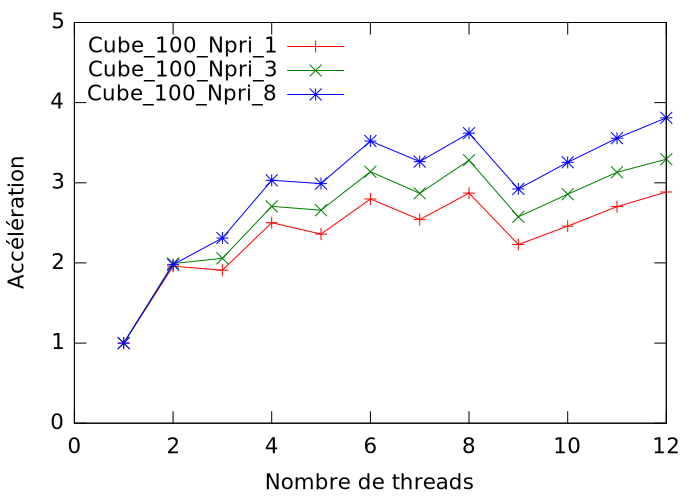
\includegraphics[width=0.7\textwidth]{res_spmv_mpi}
  \caption{Accélération du produit matrice vecteur creux sur Rostand en mémoire distribuée.}
  \label{fig:res_spmv_mpi_rostand}
\end{figure}



Sur Manumanu, nous avons beaucoup plus de banc NUMA, ce qui signifie que nous aurons plus de bande passante mémoire à notre disposition.
%
Nous pouvons donc espérer avoir de meilleurs résultats que sur Rostand.
%
Il faut aussi prendre en compte une bande passante mémoire plus élevée sur les bancs NUMA de Manumanu que sur ceux de Rostand.
%
Les processus MPI sont alloués en mode compact, c'est à dire qu'ils sont distribués de façon à utiliser un minimum de noeuds NUMA.
%
Sur 1 banc NUMA, nous avons une accélération de 5 avec 8 variables primaires (Fig.~\ref{fig:res_spmv_mpi_manumanu}).
%
Cette accélération monte à 110 avec l'utilisation des 20 bancs NUMA et des 160 coeurs.


%   (-_-)   %
\begin{figure}
  \centering
  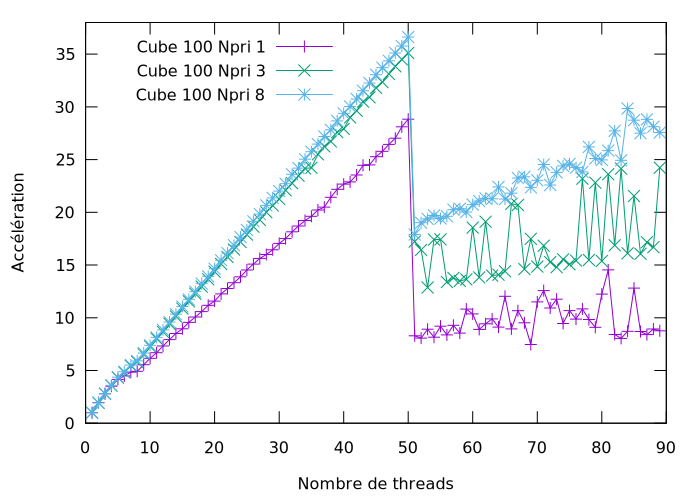
\includegraphics[width=0.7\textwidth]{res_spmv_mpi_manu}
  \caption{Accélération du produit matrice vecteur creux sur Manumanu en mémoire distribuée.}
  \label{fig:res_spmv_mpi_manumanu}
\end{figure}
